\documentclass{article}
\usepackage[utf8]{inputenc}
\usepackage{amsmath}
\usepackage{amssymb}
\usepackage{geometry}
\usepackage{graphicx}
\geometry{a4paper}

\title{Lösungen zum Übungsblatt 1}
\author{}
\date{Sommersemester 2024}

\begin{document}

\maketitle

\section*{Aufgabe P1}
\subsection*{a) Ergebnisraum}
Geeigneter Ergebnisraum für das Werfen zweier nicht unterscheidbarer Würfel ist $\{ (i, j) : 1 \leq i \leq j \leq 6 \}$. Dieser berücksichtigt, dass die Würfel nicht unterscheidbar sind und vermeidet doppelte Kombinationen wie (1,2) und (2,1).

\subsection*{b) Laplace-Annahme}
Die Laplace-Annahme ist sinnvoll, da jeder Wurf gleich wahrscheinlich ist. Da die Würfel fair sind, hat jedes mögliche Paar (i, j) die gleiche Wahrscheinlichkeit.

\subsection*{c) Ereignisse}
\begin{itemize}
    \item $A1 = E \cap F$: Das Ereignis, dass die Augensumme ungerade ist und mindestens einer der Würfel eine 3 zeigt.
    \item $A2 = F \cup G$: Mindestens einer der Würfel zeigt eine 3 oder die Augensumme ist 7.
    \item $A3 = (E \cup F) \cap G$: Die Augensumme ist 7 und zusätzlich ist entweder die Augensumme ungerade oder mindestens ein Würfel zeigt eine 3.
    \item $A4 = E \cup (F \cap G)$: Die Augensumme ist ungerade oder mindestens ein Würfel zeigt eine 3 und die Augensumme ist 7.
    \item $A5 = G \setminus E$: Die Augensumme ist 7, aber nicht ungerade.
    \item $A6 = E \cap F \cap G$: Die Augensumme ist ungerade, mindestens einer der Würfel zeigt eine 3, und die Augensumme ist 7.
\end{itemize}

\section*{Aufgabe P2}
To prove that \( A \cup B = A \cup (\neg A \cap B) \):

\textbf{Step 1:} \( A \cup B \subseteq A \cup (\neg A \cap B) \)

Let \( x \in A \cup B \). This implies \( x \in A \) or \( x \in B \). Therefore:
\begin{itemize}
  \item If \( x \in A \), then \( x \in A \cup (\neg A \cap B) \).
  \item If \( x \notin A \) but \( x \in B \), then \( x \in \neg A \) and \( x \in \neg A \cap B \), thus \( x \in A \cup (\neg A \cap B) \).
\end{itemize}

\textbf{Step 2:} \( A \cup (\neg A \cap B) \subseteq A \cup B \)

Let \( x \in A \cup (\neg A \cap B) \). This implies \( x \in A \) or \( x \in (\neg A \cap B) \). Therefore:
\begin{itemize}
  \item If \( x \in A \), then \( x \in A \cup B \).
  \item If \( x \in (\neg A \cap B) \), this implies \( x \in \neg A \) and \( x \in B \), hence \( x \in A \cup B \).
\end{itemize}

\textbf{Conclusion:}

Since \( A \cup B \subseteq A \cup (\neg A \cap B) \) and \( A \cup (\neg A \cap B) \subseteq A \cup B \), we have:
\[ A \cup B = A \cup (\neg A \cap B) \]

\section*{Aufgabe H1}
Mengen im Ergebnisraum $\Omega = [-1, 1]^2$.
\begin{itemize}
    \item $\neg A$: $\{(x, y) \in \Omega : x + y < 0\}$ 
    \[(\neg A)\]
    \begin{figure}[!ht]
        \centering
        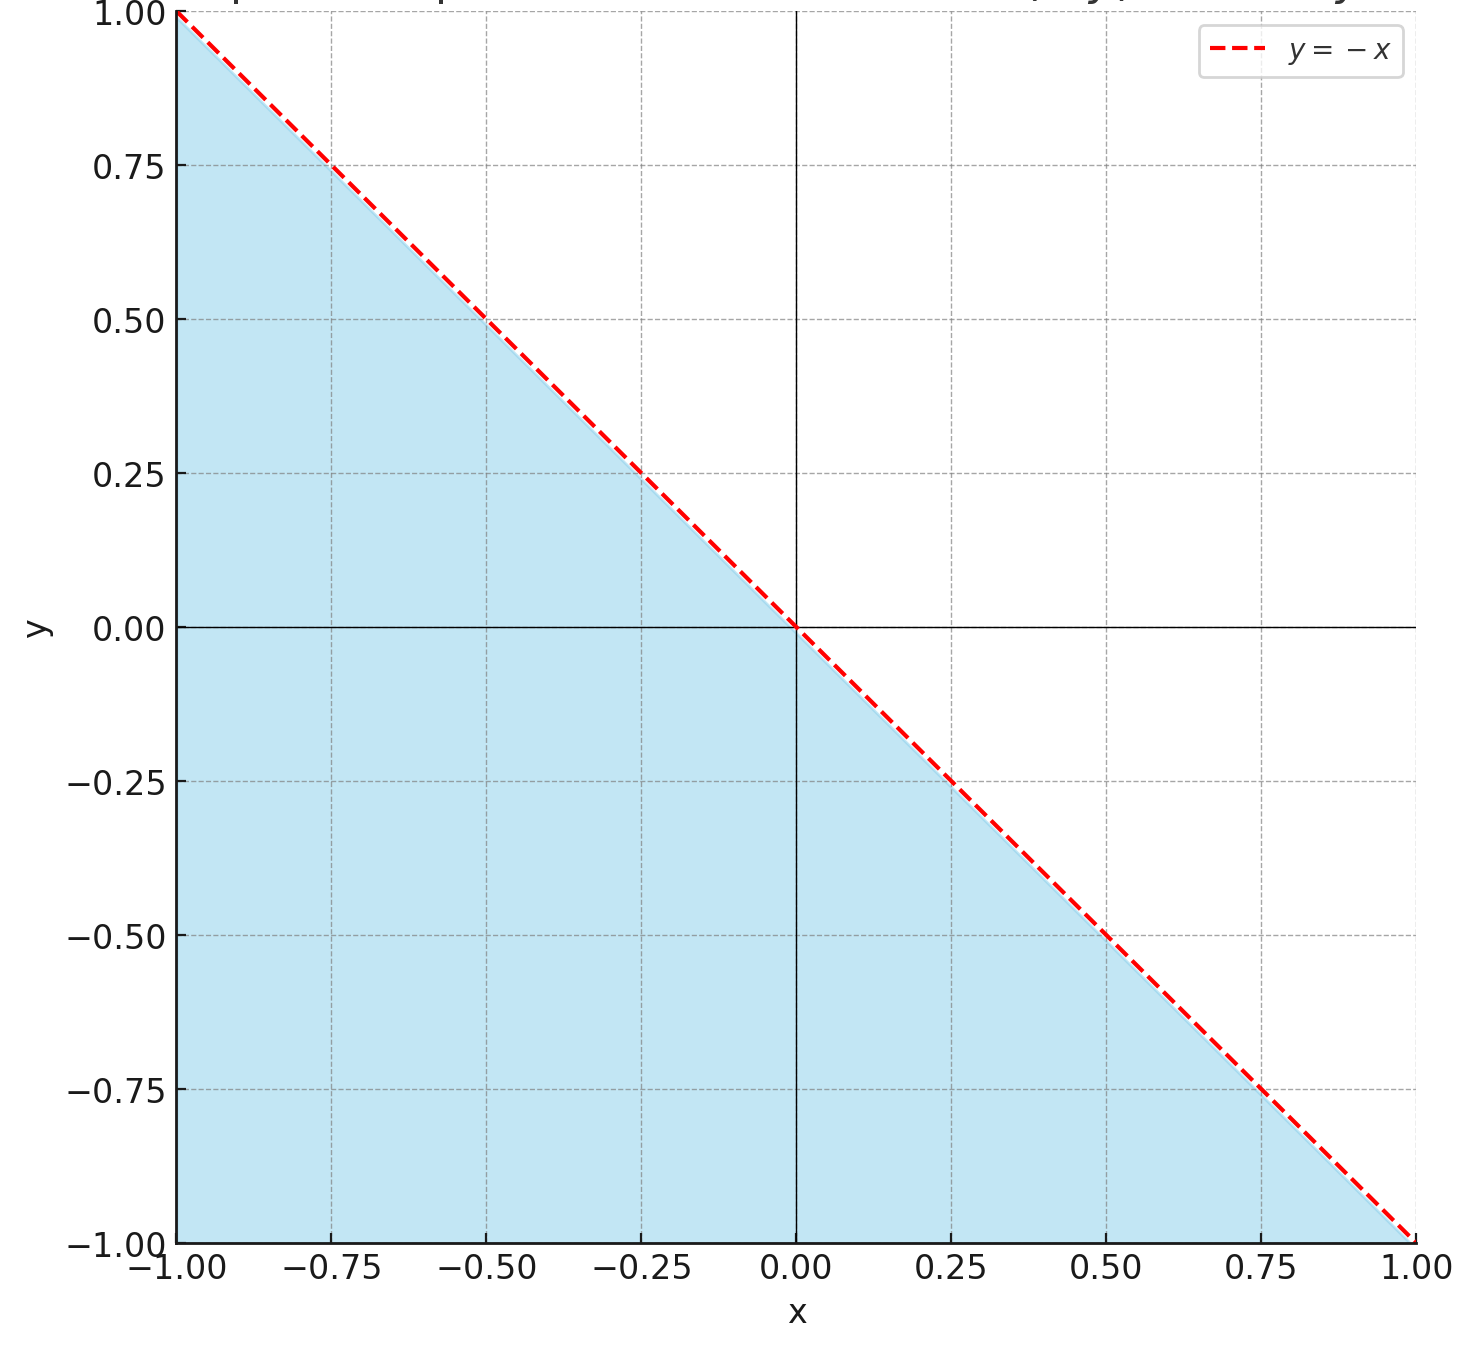
\includegraphics[width=0.8\textwidth]{img/h1_a.png}
        \caption{Graphical representation of the set \( A \) where \( x + y < 0 \).}
    \end{figure}
    \item $A \cap B$: $\{(x, y) \in \Omega : x + y \geq 0 \text{ und } |x| + |y| \geq 1\}$
    \begin{figure}[!ht]
        \centering
        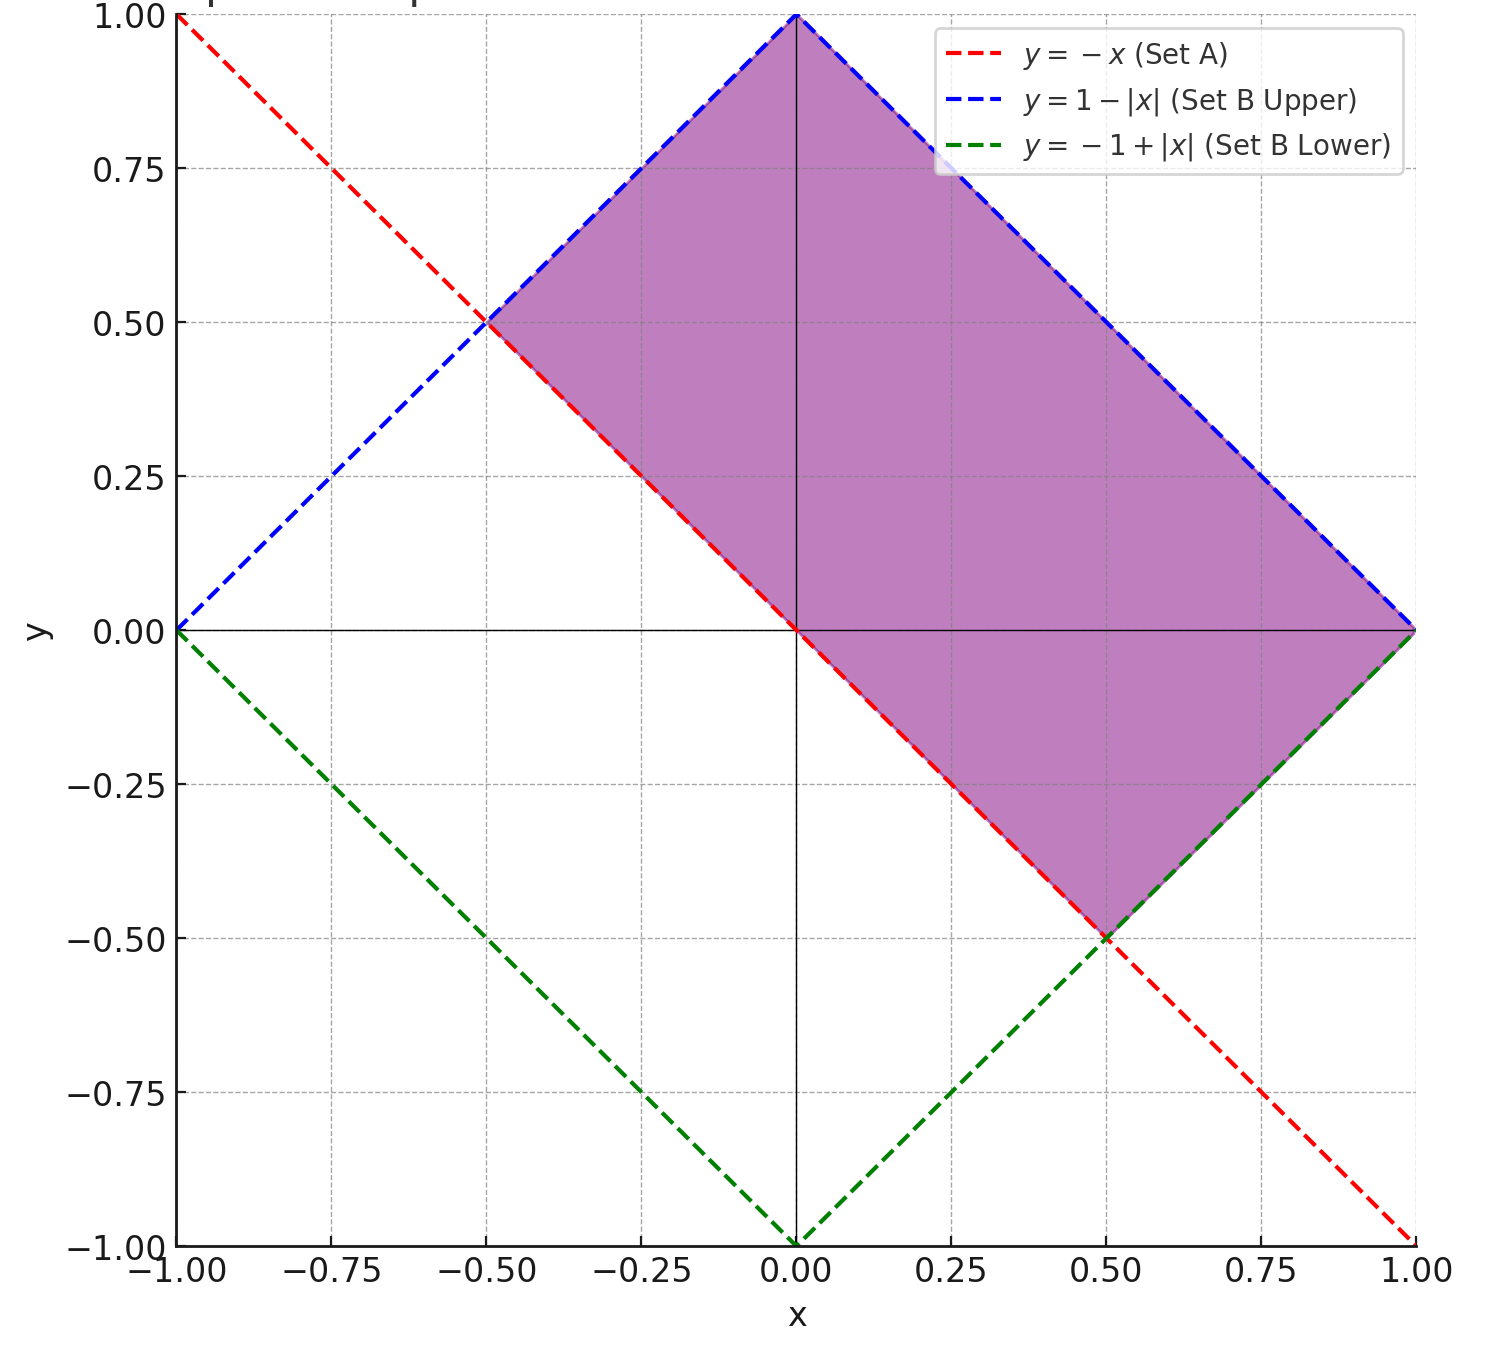
\includegraphics[width=0.8\textwidth]{img/h1_b.png}
        \caption{Description...}
    \end{figure}
    \item $(B \cup C)^c$: $\{(x, y) \in \Omega : |x| + |y| < 1 \text{ oder } x^2 < y\}$
    \begin{figure}[!ht]
        \centering
        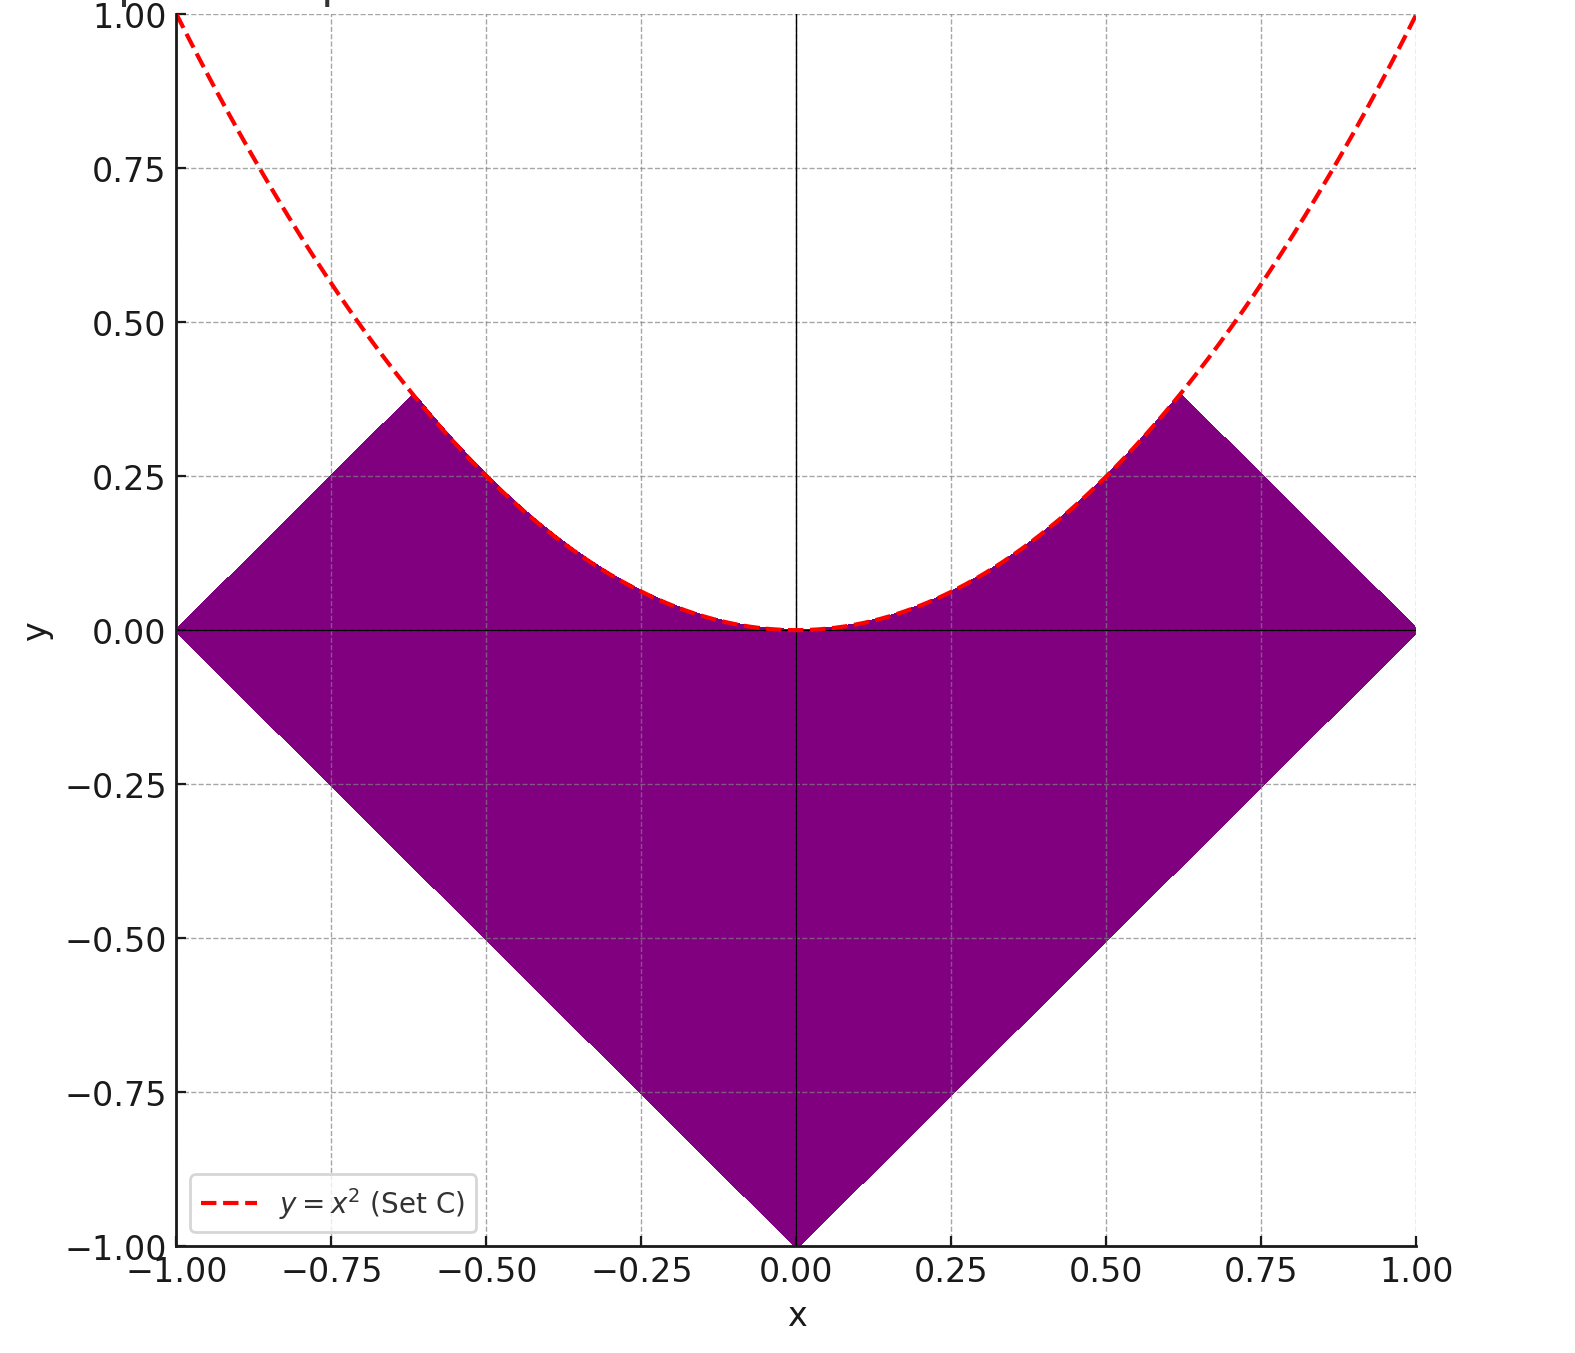
\includegraphics[width=0.8\textwidth]{img/h1_c.png}
        \caption{Description...}
    \end{figure}
\end{itemize}

\section*{Aufgabe H2}
Beweis der Gesetze von de Morgan unter Verwendung einer beliebigen Indexmenge $I$.
\begin{align*}
    \bigcup_{i \in I} A_i &= \bigcap_{i \in I} \overline{A_i} \\
    \bigcap_{i \in I} A_i &= \bigcup_{i \in I} \overline{A_i}
\end{align*}

\end{document}
